\section{Results}
\label{sec:results}

\subsection{In-dataset results look excellent}

\begin{table*}[t]
\centering
\small
\begin{tabular}{lccccccccc}
\toprule
& \multicolumn{3}{c}{UNSW-NB15} & \multicolumn{3}{c}{ToN-IoT} & \multicolumn{3}{c}{CIC-IDS2018} \\
\cmidrule(lr){2-4}\cmidrule(lr){5-7}\cmidrule(lr){8-10}
Model & F1 & Recall & FPR & F1 & Recall & FPR & F1 & Recall & FPR \\
\midrule
\inputrows tab_indataset.tex 
\bottomrule
\end{tabular}
\caption{In-dataset results, where each model is trained and tested on the same dataset. Values are means over three seeds. FPR is the share of benign flows flagged as attacks.}
\label{tab:indataset}
\end{table*}

Table~\ref{tab:indataset} shows the usual in-dataset setting, where each model is trained and tested on splits of the same dataset. Every model looks like a working intrusion detector here. F1 ranges from \INFMIN{} to \INFMAX{}, recall is above 0.9 everywhere, and most false positive rates are below 1 percent. The random forest is the best model on every dataset. False positive rates are higher on ToN-IoT for every model, and highest for logistic regression, which flags 15.4 percent of benign flows there. If this were the only experiment, the natural conclusion would be that the problem is mostly solved and the random forest is the model to use.

\subsection{Performance collapses on new networks}

\begin{figure*}[t]
\centering
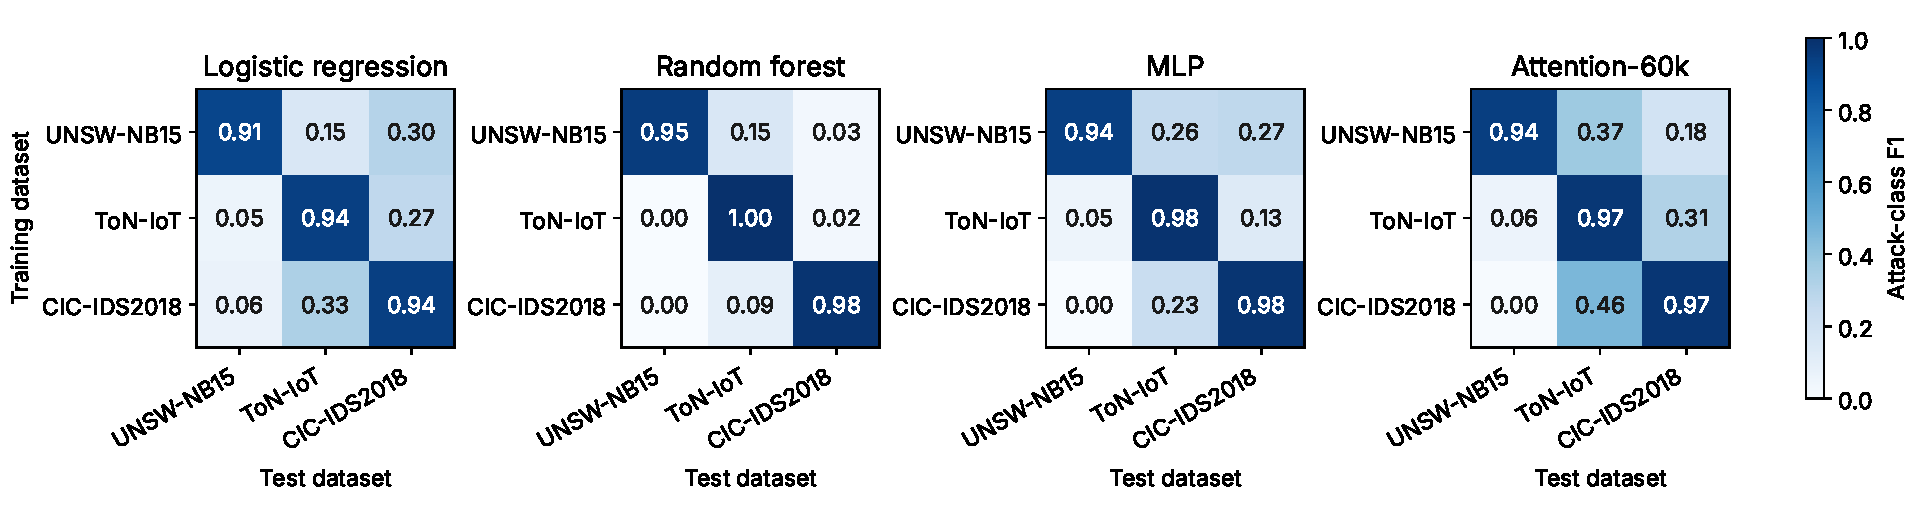
\includegraphics[width=\linewidth]{fig_matrix.pdf}
\caption{Attack-class F1 for every pair of training and test dataset, averaged over three seeds. The diagonal is the in-dataset result. Every off-diagonal cell is a model tested on a network it never saw during training. The attention model was trained on 60,000 flows per source, as described in Section~\ref{sec:method}.}
\label{fig:matrix}
\end{figure*}

\begin{table*}[t]
\centering
\small
\begin{tabular}{lcccccccc}
\toprule
& \multicolumn{3}{c}{F1} & \multicolumn{2}{c}{ROC AUC} & \multicolumn{3}{c}{Cross-dataset} \\
\cmidrule(lr){2-4}\cmidrule(lr){5-6}\cmidrule(lr){7-9}
Model & In-dataset & Cross-dataset & Gap & In-dataset & Cross-dataset & Recall & FPR & Accuracy \\
\midrule
\inputrows tab_summary.tex 
\bottomrule
\end{tabular}
\caption{Summary of single-source transfer. In-dataset values average the three diagonal cells of Figure~\ref{fig:matrix} and cross-dataset values average the six off-diagonal cells, over three seeds. The gap is in-dataset F1 minus cross-dataset F1.}
\label{tab:summary}
\end{table*}

Figure~\ref{fig:matrix} and Table~\ref{tab:summary} show what happens when the test data comes from a different network. Every model falls apart. Averaged over the six cross-dataset pairs, F1 is 0.194 for logistic regression, 0.157 for the MLP, and 0.049 for the random forest. \ATTNCROSS{} No model reaches an F1 above \CROSSMAX{} on any network it was not trained on.

The way the models fail depends on the pair of datasets. Some models flag almost everything. Logistic regression trained on ToN-IoT flags 93.7 percent of the benign flows in UNSW-NB15 and 72.8 percent of the benign flows in CIC-IDS2018. Other models flag almost nothing. The random forest trained on CIC-IDS2018 catches 0 of the attacks in UNSW-NB15, and the random forest trained on ToN-IoT catches 0.3 percent. A deployed detector that floods operators with false alarms and a detector that stays silent during an attack are both useless, and the same models do both depending on where they are moved.

\subsection{Accuracy, F1, and AUC can all mislead}

\FLAGPARA

Accuracy makes several of these failures look fine. The random forest trained on CIC-IDS2018 has an accuracy of 96.0 percent on UNSW-NB15 while detecting no attacks at all, because about 96 percent of UNSW-NB15 is benign and the model labels nearly everything benign. The random forest also has the highest average cross-dataset accuracy in Table~\ref{tab:summary}, at 0.649, even though it has the lowest cross-dataset F1. This is the base rate problem described by Arp \etal \cite{arp2022}, and it is why this project uses attack-class F1 as the main metric.

ROC AUC is not a safe summary either. It does not depend on the threshold, so it could have shown that the models still rank flows correctly and only need a new threshold. That is not what happened. Cross-dataset AUC was at or below 0.5 in 2 of the 6 cross-dataset cells for logistic regression, 3 for the MLP, and 4 for the random forest, with a lowest value of 0.217 for the random forest trained on ToN-IoT and tested on UNSW-NB15. An AUC below 0.5 means the model ranks benign flows as more suspicious than attacks. Recalibrating the threshold on the new network would not fix these models, because what they learned points the wrong way.

\subsection{More complex models do not generalize better}

The ranking of the models flips between the two settings. The random forest is the best model in-dataset, with an average F1 of 0.977 and an average AUC of 0.996. It is the worst model across datasets, with an average cross-dataset AUC of 0.413. Logistic regression is the weakest model in-dataset and has the second smallest gap, 0.736, just behind the attention model discussed next. This supports the hypothesis from the proposal that more flexible models would score higher in-dataset without generalizing better. A model with more capacity can fit the specific patterns of one lab more closely, and those are exactly the patterns that do not carry over.

\ATTNPARA

\subsection{Training on two networks does not close the gap}

\begin{table*}[t]
\centering
\small
\resizebox{\linewidth}{!}{\begin{tabular}{lcccccccc}
\toprule
& \multicolumn{2}{c}{Held out UNSW-NB15} & \multicolumn{2}{c}{Held out ToN-IoT} & \multicolumn{2}{c}{Held out CIC-IDS2018} & \multicolumn{2}{c}{Average} \\
\cmidrule(lr){2-3}\cmidrule(lr){4-5}\cmidrule(lr){6-7}\cmidrule(lr){8-9}
Model & One source & Two sources & One source & Two sources & One source & Two sources & One source & Two sources \\
\midrule
\inputrows tab_multi.tex 
\bottomrule
\end{tabular}}
\caption{Attack-class F1 on a held-out dataset. One source is the average F1 of the two single-source models trained on the other datasets. Two sources is the model trained on both of those datasets combined. \MULTICAPTION}
\label{tab:multi}
\end{table*}

\begin{figure*}[t]
\centering
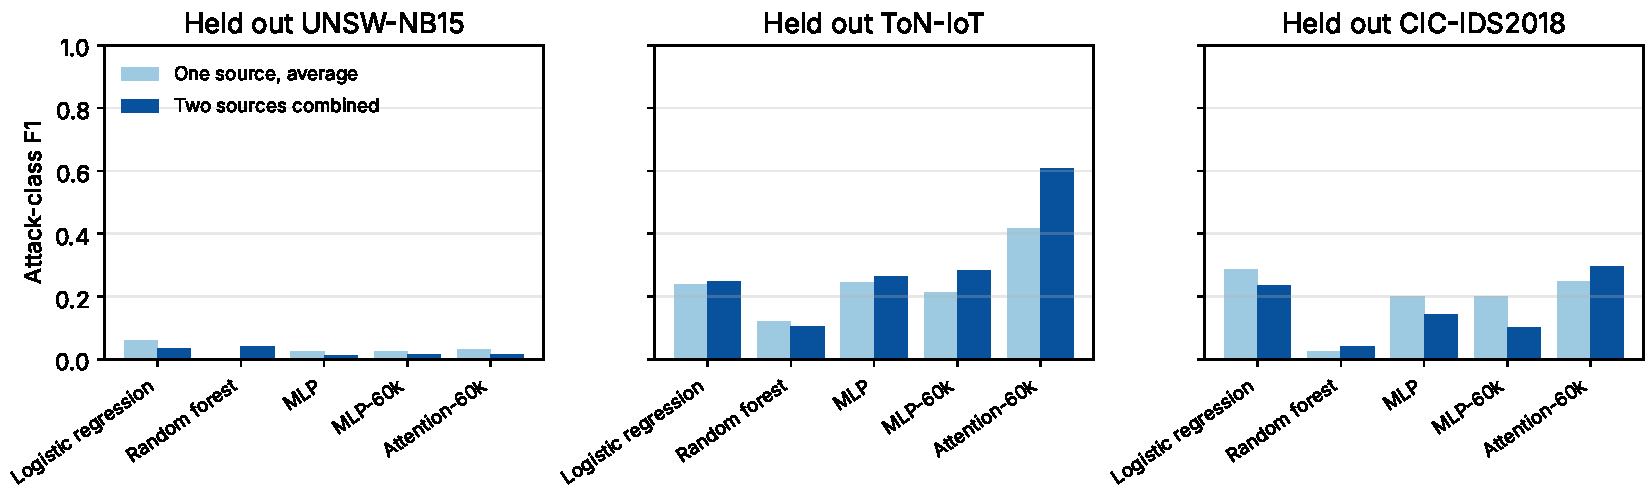
\includegraphics[width=0.9\linewidth]{fig_multi.pdf}
\caption{Held-out F1 with one training source, averaged over the two possible sources, and with both sources combined.}
\label{fig:multi}
\end{figure*}

The proposal expected that training on more than one network would shrink the gap without closing it. Table~\ref{tab:multi} and Figure~\ref{fig:multi} show that it barely shrinks it at all. Averaged over the three held-out datasets, the held-out F1 of logistic regression goes from 0.194 with one source to 0.173 with two, and the MLP goes from 0.157 to 0.139. The random forest goes from 0.049 to 0.061. None of these changes is large enough to matter, and two of them go the wrong way. \MULTIATTN

The reason shows up when the multi-source models are tested on the two networks they were trained on. The random forest still gets an average F1 of 0.976 on those two networks and the MLP gets 0.965, almost the same as their single-source in-dataset scores. Both models are flexible enough to learn a separate rule for each network instead of finding what the attacks have in common. A third network gets neither rule. Logistic regression cannot do this, and its F1 on its own two training networks drops to 0.748. A single linear boundary cannot fit both networks at once, which is more evidence that the networks really are different problems.

\subsection{What the models rely on}
\label{sec:features}

\begin{table*}[t]
\centering
\small
\resizebox{\linewidth}{!}{\begin{tabular}{llllllll}
\toprule
Model & Trained on & First & Drop & Second & Drop & Third & Drop \\
\midrule
\inputrows tab_features.tex
\bottomrule
\end{tabular}}
\caption{The three most important features for each in-dataset model by permutation importance. Drop is the average fall in ROC AUC on the model's own test set when that feature is shuffled.}
\label{tab:features}
\end{table*}

\begin{table}[t]
\centering
\small
\resizebox{\columnwidth}{!}{\begin{tabular}{lll}
\toprule
Dataset & Benign MIN\_TTL & Attack MIN\_TTL \\
\midrule
UNSW-NB15 & 31 in 98.4\% & 254 in 75.2\%, 62 in 24.6\% \\
ToN-IoT & 0 in 84.6\% & 0 in 52.8\%, 64 in 46.1\% \\
CIC-IDS2018 & 0 in 40.7\% & 127 in 61.2\%, 63 in 26.7\% \\
\bottomrule
\end{tabular}}
\caption{Most common MIN\_TTL values in each sample, split by class.}
\label{tab:ttl}
\end{table}

Table~\ref{tab:features} lists the most important features for the random forest and the MLP on each dataset. The two models trained on UNSW-NB15 both rank the TTL features near the top. On ToN-IoT both models depend heavily on L7\_PROTO, the layer 7 protocol ID. Shuffling it alone lowers the random forest's AUC by 0.111. The MLP trained on CIC-IDS2018 leans mostly on TCP\_FLAGS. The random forest's importance values are small in general, because it can usually fall back on another feature that carries the same information when one is shuffled.

The more important point is that the models learn different rules on each network. The Spearman rank correlation between the MLP's feature importance on two different datasets is only between \SPMLPMIN{} and \SPMLPMAX{}, so a feature that matters on one network says little about whether it matters on another. The benign traffic itself is also very different. For each feature, a two-sample Kolmogorov-Smirnov statistic was computed between the benign flows of every pair of datasets. The median feature has an average statistic of \KSMED{}, and \KSSHARE{} percent of the features are above 0.5. Normal traffic on one network does not look like normal traffic on another, which is the diversity problem Sommer and Paxson described \cite{sommer2010}.

The TTL features are the clearest example of a lab artifact. Table~\ref{tab:ttl} shows that 98.4 percent of the benign flows in the UNSW-NB15 sample have a minimum TTL of exactly 31, while almost every attack has a TTL of 254 or 62. TTL depends mostly on the operating system that sent the packet and on how many routers it crossed, so these values describe the machines and layout of the UNSW lab and not the attacks. To check how strong this shortcut is, a single rule that labels a flow as an attack whenever its minimum TTL is not 31 was tested. On the UNSW-NB15 test split this rule gets 100 percent recall, a false positive rate of 1.7 percent, and an F1 of 0.832 without any learning. On ToN-IoT and CIC-IDS2018 the same rule flags every single flow. This is the spurious correlation pitfall from Arp \etal \cite{arp2022}, sitting inside one of the most widely used benchmark datasets.

\subsection{Removing the TTL shortcut}

\begin{table}[t]
\centering
\small
\setlength{\tabcolsep}{4pt}
\resizebox{\columnwidth}{!}{\begin{tabular}{lcccccc}
\toprule
& \multicolumn{2}{c}{UNSW in} & \multicolumn{2}{c}{UNSW out} & \multicolumn{2}{c}{All cross} \\
\cmidrule(lr){2-3}\cmidrule(lr){4-5}\cmidrule(lr){6-7}
Model & TTL & No TTL & TTL & No TTL & TTL & No TTL \\
\midrule
\inputrows tab_ablation.tex
\bottomrule
\end{tabular}}
\caption{Attack-class F1 with and without the two TTL features. UNSW in is trained and tested on UNSW-NB15. UNSW out is trained on UNSW-NB15 and averaged over the other two test sets. All cross averages all six cross-dataset pairs.}
\label{tab:ablation}
\end{table}

\ABLATIONPARA

\subsection{Stability across seeds}

In-dataset results barely change between seeds, with F1 moving by less than 0.01 for every model. Cross-dataset results are much less stable. The random forest trained on UNSW-NB15 and tested on ToN-IoT gets an F1 of 0.077, 0.329, and 0.047 for the three seeds. When the test data looks nothing like the training data, small changes in how the model is built decide which wrong rule it ends up using. This is one more reason a single cross-dataset number should not be trusted on its own.
